\documentclass{ximera}
\usepackage{OERLinearAlgebra}


\usepackage{mathtools}
\usepackage{tikz-3dplot}
\usetikzlibrary{shapes.geometric}
\usetikzlibrary{arrows}

\author{Anna Davis \and Paul Zachlin} \title{Span} \license{CC-BY 4.0}

\begin{document}

\begin{abstract}
 We define span and introduce the idea of redundant vectors.
\end{abstract}
\maketitle


\section*{Motivation}
%In the previous section we considered different ways for determining whether one given vector is a linear combination of a collection of vectors.  In this section, we consider the set of all linear combinations of a collection of vectors.

Recall that a vector $\vec{v}$ is said to be a linear combination of vectors $\vec{v}_1, \vec{v}_2,\ldots, \vec{v}_n$ if 
$$\vec{v}=a_1\vec{v}_1+ a_2\vec{v}_2+\ldots + a_n\vec{v}_n$$
for some scalars $a_1, a_2, \ldots ,a_n$.


\begin{example}\label{ex:spanintro}
If possible, express the given vector as a linear combination of $$\vec{v}_1=\begin{bmatrix}-2\\-3\\4\end{bmatrix},\quad\vec{v}_2=\begin{bmatrix}2\\3\\2\end{bmatrix}$$  Interpret your results geometrically.

  \begin{enumerate}
  \item \label{item:spanintro1} 
  $$\vec{u}=\begin{bmatrix}2\\3\\5\end{bmatrix}$$
  
  
  \item \label{item:spanintro2}
  $$\vec{w}=\begin{bmatrix}5\\5\\1\end{bmatrix}$$
  \end{enumerate}
  
  \begin{explanation}
  \ref{item:spanintro1} We need to find coefficients $a_1$ and $a_2$ such that $\vec{u}=a_1\vec{v}_1+a_2\vec{v}_2$. To do this we need to solve the vector equation:
  $$a_1\begin{bmatrix}-2\\-3\\4\end{bmatrix}+a_2\begin{bmatrix}2\\3\\2\end{bmatrix}=\begin{bmatrix}2\\3\\5\end{bmatrix}$$
  This equation translates into the following system:
  
  $$\begin{array}{ccccc}
      -2a_1 & +&2a_2&= &2 \\
        -3a_1& +&3a_2&= &3 \\
      4a_1 &+ &2a_2&= &5\\
	     \end{array}$$
  We write the system in augmented matrix form and apply elementary row operations to bring it to reduced row-echelon form.
  $$\left[\begin{array}{cc|c}  
 -2&2&2\\-3&3&3\\4&2&5
 \end{array}\right]\rightsquigarrow\left[\begin{array}{cc|c}  
 1&0&1/2\\0&1&3/2\\0&0&0
 \end{array}\right]$$
  
  This shows that $a_1=\frac{1}{2}$ and $a_2=\frac{3}{2}$, and we can express $\vec{u}$ as a linear combination of $\vec{v}_1$ and $\vec{v}_2$ as follows:
  $$\frac{1}{2}\begin{bmatrix}-2\\-3\\4\end{bmatrix}+\frac{3}{2}\begin{bmatrix}2\\3\\2\end{bmatrix}=\begin{bmatrix}2\\3\\5\end{bmatrix}$$
    
  Observe that because vector $\vec{u}$ is a linear combination of $\vec{v}_1$ and $\vec{v}_2$, $\vec{u}$ is the diagonal of a parallelogram whose sides are scalar multiples of $\vec{v}_1$ and $\vec{v}_2$. As such, $\vec{u}$ lies in the same plane as $\vec{v}_1$ and $\vec{v}_2$, as illustrated below.
  
  \begin{image}
\tdplotsetmaincoords{70}{130}
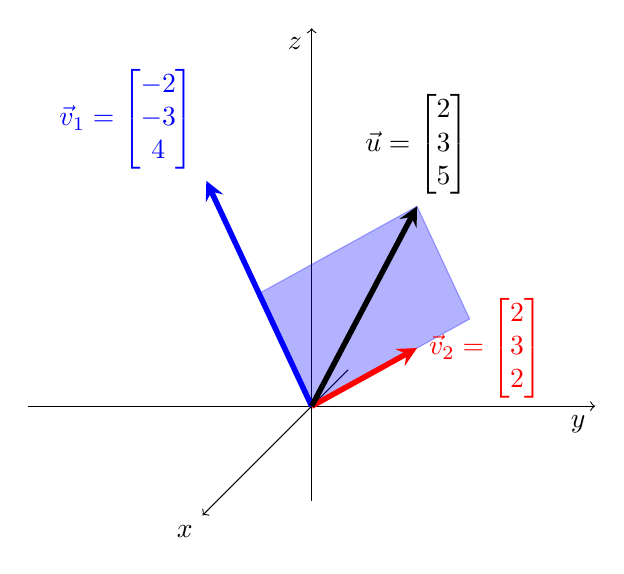
\begin{tikzpicture}[scale=0.6]
	\draw[->](-6,0,0)--(6,0,0) node[below left]{$y$};
    \draw[->](0,-2,0)--(0,8,0) node[below left]{$z$};
    \draw[->](0,0,-2)--(0,0,6) node[below left]{$x$};
    
    \filldraw[blue, opacity=0.3](0,0,0)--(4.5,3,3)--(3,5,2)--(-1.5,2,-1)--cycle;
    \draw[->, line width=2pt,blue, -stealth](0,0,0)--(-3,4,-2)node[above left]{$\vec{v}_1=\begin{bmatrix}-2\\-3\\4\end{bmatrix}$};
    \draw[->, line width=2pt,red, -stealth](0,0,0)--(3,2,2)node[right]{$\vec{v}_2=\begin{bmatrix}2\\3\\2\end{bmatrix}$};
    \draw[->, line width=2pt, -stealth](0,0,0)--(3,5,2)node[above]{$\vec{u}=\begin{bmatrix}2\\3\\5\end{bmatrix}$};
    
    \end{tikzpicture}
\end{image}
  
  
%We say that $\vec{u}$ is \dfn{in the span of} $\vec{v}_1$ and $\vec{v}_2$.
  
  
\ref{item:spanintro2}  
We need to solve the following vector equation:   $$a_1\begin{bmatrix}-2\\-3\\4\end{bmatrix}+a_2\begin{bmatrix}2\\3\\2\end{bmatrix}=\begin{bmatrix}5\\5\\1\end{bmatrix}$$
  This equation corresponds to the system:
  
  $$\begin{array}{ccccc}
      -2a_1 & +&2a_2&= &5 \\
        -3a_1& +&3a_2&= &5 \\
      4a_1 &+ &2a_2&= &1\\
	     \end{array}$$
  Writing the system in augmented matrix form and applying elementary row operations gives us the following reduced row-echelon form:
  $$\left[\begin{array}{cc|c}  
 -2&2&5\\-3&3&5\\4&2&1
 \end{array}\right]\rightsquigarrow\left[\begin{array}{cc|c}  
 1&0&0\\0&1&0\\0&0&1
 \end{array}\right]$$
 We conclude that there are no solutions, and $\vec{w}$ is not a linear combination of $\vec{v}_1$ and $\vec{v}_2$.
 
 Geometrically, this means that $\vec{w}$ is not the diagonal of any parallelogram whose sides are scalar multiples of $\vec{v}_1$ and $\vec{v}_2$.  Thus, $\vec{w}$ does not lie in the plane determined by $\vec{v}_1$ and $\vec{v}_2$.  
 %We say that $\vec{w}$ is not \dfn{in the span} of $\vec{v}_1$ and $\vec{v}_2$.
 
  \begin{image}
\tdplotsetmaincoords{70}{130}
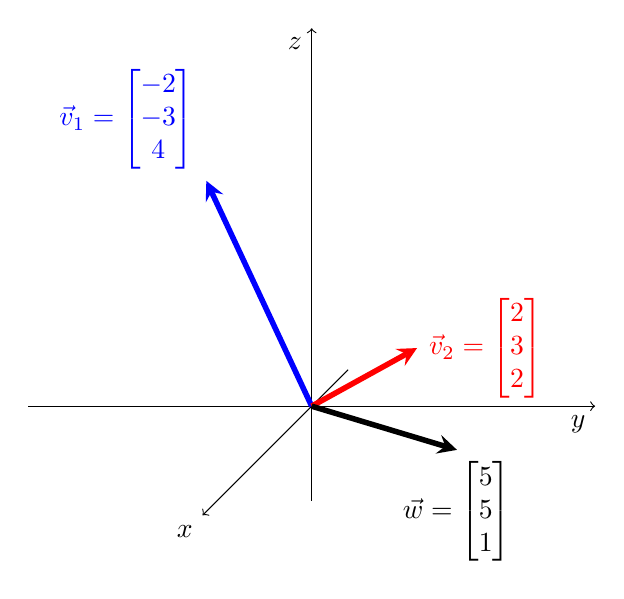
\begin{tikzpicture}[scale=0.6]
	\draw[->](-6,0,0)--(6,0,0) node[below left]{$y$};
    \draw[->](0,-2,0)--(0,8,0) node[below left]{$z$};
    \draw[->](0,0,-2)--(0,0,6) node[below left]{$x$};
    
    
    \draw[->, line width=2pt,blue, -stealth](0,0,0)--(-3,4,-2)node[above left]{$\vec{v}_1=\begin{bmatrix}-2\\-3\\4\end{bmatrix}$};
   
   \draw[->, line width=2pt,red, -stealth](0,0,0)--(3,2,2)node[right]{$\vec{v}_2=\begin{bmatrix}2\\3\\2\end{bmatrix}$};
    
    \draw[->, line width=2pt, -stealth](0,0,0)--(5,1,5)node[below]{$\vec{w}=\begin{bmatrix}5\\5\\1\end{bmatrix}$};

\end{tikzpicture}
\end{image}
  
  \end{explanation}
\end{example}

In part \ref{item:spanintro1} of Example \ref{ex:spanintro} we expressed $\vec{u}$ as a linear combination of $\vec{v}_1$ and $\vec{v}_2$, and concluded that $\vec{u}$ lies in the plane determined by $\vec{v}_1$ and $\vec{v}_2$.  We will now introduce a new vocabulary term and say that $\vec{u}$ is \dfn{in the span} of $\vec{v}_1$ and $\vec{v}_2$.  

In contrast, vector $\vec{w}$ of part \ref{item:spanintro2} of Example \ref{ex:spanintro} is not a linear combination of $\vec{v}_1$ and $\vec{v}_2$.  We say that $\vec{w}$ is not in the span of $\vec{v}_1$ and $\vec{v}_2$.

\section*{Definition of Span}

\begin{definition}\label{def:span} Let $\vec{v}_1, \vec{v}_2,\ldots ,\vec{v}_p$ be vectors in $\RR^n$.  The set $S$ of all linear combinations of $\vec{v}_1, \vec{v}_2,\ldots ,\vec{v}_p$ is called the span of $\vec{v}_1, \vec{v}_2,\ldots ,\vec{v}_p$.  We write 
$$S=\textnormal{span}(\vec{v}_1, \vec{v}_2,\ldots ,\vec{v}_p)$$
and we say that vectors $\vec{v}_1, \vec{v}_2,\ldots ,\vec{v}_p$ span $S$.  Any vector in $S$ is said to be in the span of $\vec{v}_1, \vec{v}_2,\ldots ,\vec{v}_p$.  The set $\{\vec{v}_1, \vec{v}_2,\ldots ,\vec{v}_p\}$ is called the \dfn{spanning set} for $S$.
\end{definition}

\begin{example}
Describe $\textnormal{span}\left(\begin{bmatrix}-3\\1\end{bmatrix}\right)$.
\begin{explanation}
The span of $\begin{bmatrix}-3\\1\end{bmatrix}$ is the set of all linear combinations of $\begin{bmatrix}-3\\1\end{bmatrix}$.  Since we are looking for linear combinations of only one vector, we are really looking for all of its scalar multiples.  So, the span will be the set of all vectors of the form $\vec{v}=a\begin{bmatrix}-3\\1\end{bmatrix}$.  All such vectors lie on the line determined by $\begin{bmatrix}-3\\1\end{bmatrix}$.

\begin{image}[3.5in]
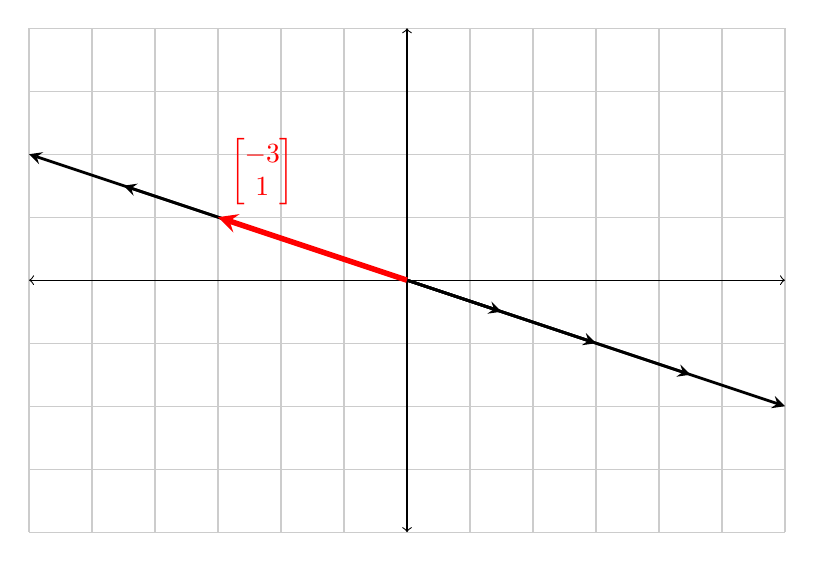
\begin{tikzpicture}[scale=0.8]
\draw[thin,gray!40] (-6,-4) grid (6,4);
  \draw[<->] (-6,0)--(6,0);
  \draw[<->] (0,-4)--(0,4);
  
 \draw[line width=1pt,-stealth](0,0)--(-6,2);
 \draw[line width=1pt,-stealth](0,0)--(6,-2);
 \draw[line width=1pt,-stealth](0,0)--(3,-1);
 \draw[line width=1pt,-stealth](0,0)--(1.5,-0.5);
 \draw[line width=1pt,-stealth](0,0)--(4.5,-1.5);
 \draw[line width=1pt,-stealth](0,0)--(-4.5,1.5);

 \draw[line width=2pt,red,-stealth](0,0)--(-3,1) node[above right]{$\begin{bmatrix}-3\\1\end{bmatrix}$};

 \end{tikzpicture}
\end{image}


\end{explanation}
\end{example}

\begin{example}
Describe $\textnormal{span}\left(\begin{bmatrix}2\\2\end{bmatrix}, \begin{bmatrix}-1\\0\end{bmatrix}\right)$.
\begin{explanation}
First, observe that $\begin{bmatrix}2\\2\end{bmatrix}$ and $\begin{bmatrix}-1\\0\end{bmatrix}$ are not scalar multiples of each other, so they do not lie on the same line.  

\begin{image}[3in]
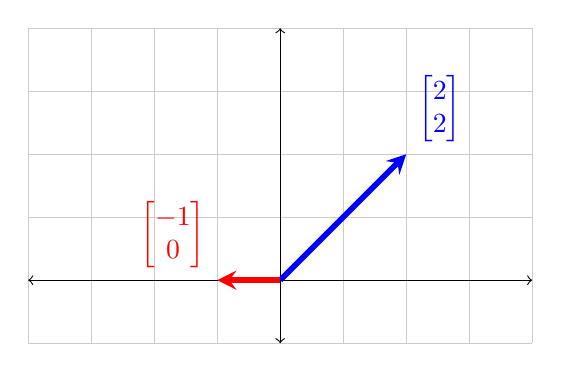
\begin{tikzpicture}[scale=0.8]
\draw[thin,gray!40] (-4,-1) grid (4,4);
  \draw[<->] (-4,0)--(4,0);
  \draw[<->] (0,-1)--(0,4);
  
  \draw[line width=2pt,blue,-stealth](0,0)--(2,2) node[above right]{$\begin{bmatrix}2\\2\end{bmatrix}$};
  \draw[line width=2pt,red,-stealth](0,0)--(-1,0) node[above left]{$\begin{bmatrix}-1\\0\end{bmatrix}$};

 \end{tikzpicture}
\end{image}


%If $\vec{w}$ is a scalar multiple of one of $\begin{bmatrix}2\\2\end{bmatrix}, \begin{bmatrix}-1\\0\end{bmatrix}$, then $\vec{w}$ is in $\textnormal{span}\left(\begin{bmatrix}2\\2\end{bmatrix}, \begin{bmatrix}-1\\0\end{bmatrix}\right)$.  
Geometrically, we can use Procedure \ref{pro:lincombgeo} of VEC-M-0040 to express any vector of $\RR^2$ as a linear combination of $\begin{bmatrix}2\\2\end{bmatrix}$ and  $\begin{bmatrix}-1\\0\end{bmatrix}$.  

To verify this claim algebraically we will show that an arbitrary vector $\begin{bmatrix}s\\t\end{bmatrix}$ of $\RR^2$ can be written as a linear combination of $\begin{bmatrix}2\\2\end{bmatrix}$ and  $\begin{bmatrix}-1\\0\end{bmatrix}$.  

Consider the vector equation:

$$a_1\begin{bmatrix}2\\2\end{bmatrix}+a_2\begin{bmatrix}-1\\0\end{bmatrix}=\begin{bmatrix}s\\t\end{bmatrix}$$
  This corresponds to the system:
  
  $$\begin{array}{ccccc}
      2a_1 & -&a_2&= &s \\
        2a_1& &&= &t \\
      
	     \end{array}$$
  Writing the system in augmented matrix form and applying elementary row operations gives us the following reduced row-echelon form:
  $$\left[\begin{array}{cc|c}  
 2&-1&s\\2&0&t
 \end{array}\right]\rightsquigarrow\left[\begin{array}{cc|c}  
 1&0&t/2\\0&1&t-s
 \end{array}\right]$$
This shows that every vector of $\RR^2$ can be written as a linear combination of $\begin{bmatrix}2\\2\end{bmatrix}$ and  $\begin{bmatrix}-1\\0\end{bmatrix}$: 

$$(t/2)\begin{bmatrix}2\\2\end{bmatrix}+(t-s)\begin{bmatrix}-1\\0\end{bmatrix}=\begin{bmatrix}s\\t\end{bmatrix}$$

We conclude that $$\textnormal{span}\left(\begin{bmatrix}2\\2\end{bmatrix}, \begin{bmatrix}-1\\0\end{bmatrix}\right)=\RR^2$$
\end{explanation}
\end{example}

\begin{example}\label{ex:spanoftwovectors}
Describe $\textnormal{span}\left(\begin{bmatrix}5\\0\\4\end{bmatrix}, \begin{bmatrix}0\\4\\2\end{bmatrix}\right)$.
\begin{explanation}
First, observe that $\begin{bmatrix}5\\0\\4\end{bmatrix}, \begin{bmatrix}0\\4\\2\end{bmatrix}$ are not scalar multiples of each other, so they do not lie on the same line.  

\begin{image}
\tdplotsetmaincoords{70}{130}
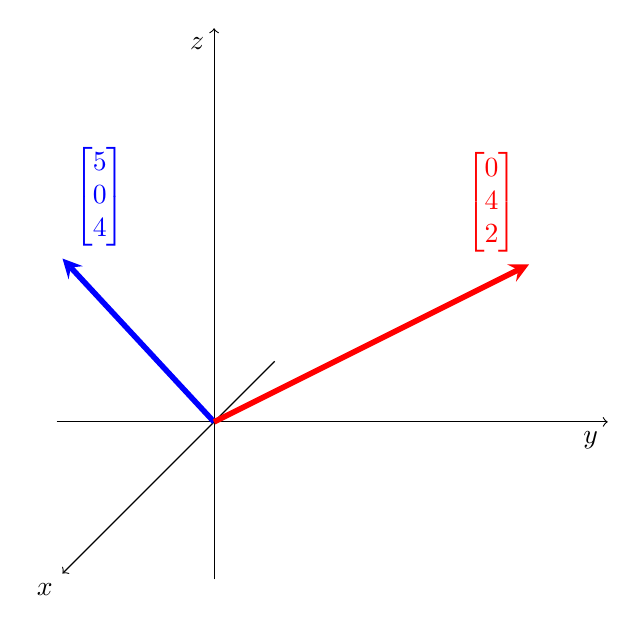
\begin{tikzpicture}
	\draw[->](-2,0,0)--(5,0,0) node[below left]{$y$};
    \draw[->](0,-2,0)--(0,5,0) node[below left]{$z$};
    \draw[->](0,0,-2)--(0,0,5) node[below left]{$x$};
    
    \draw[->, line width=2pt,blue, -stealth](0,0,0)--(0,4,5)node[above right]{$\begin{bmatrix}5\\0\\4\end{bmatrix}$};
    \draw[->, line width=2pt,red, -stealth](0,0,0)--(4,2,0)node[above left]{$\begin{bmatrix}0\\4\\2\end{bmatrix}$};
    
\end{tikzpicture}
\end{image}

The span of $\begin{bmatrix}5\\0\\4\end{bmatrix}$ and $\begin{bmatrix}0\\4\\2\end{bmatrix}$ consists of elements of the form
$$a_1\begin{bmatrix}5\\0\\4\end{bmatrix}+a_2\begin{bmatrix}0\\4\\2\end{bmatrix}$$

Geometrically, we can interpret all such linear combinations as diagonals of parallelograms determined by scalar multiples of $\begin{bmatrix}5\\0\\4\end{bmatrix}$ and $\begin{bmatrix}0\\4\\2\end{bmatrix}$.  All such diagonals will lie in the plane determined by $\begin{bmatrix}5\\0\\4\end{bmatrix}$ and $\begin{bmatrix}0\\4\\2\end{bmatrix}$.  Let this plane be called $p$.  A portion of $p$ is shown below.
\begin{image}
\tdplotsetmaincoords{70}{130}
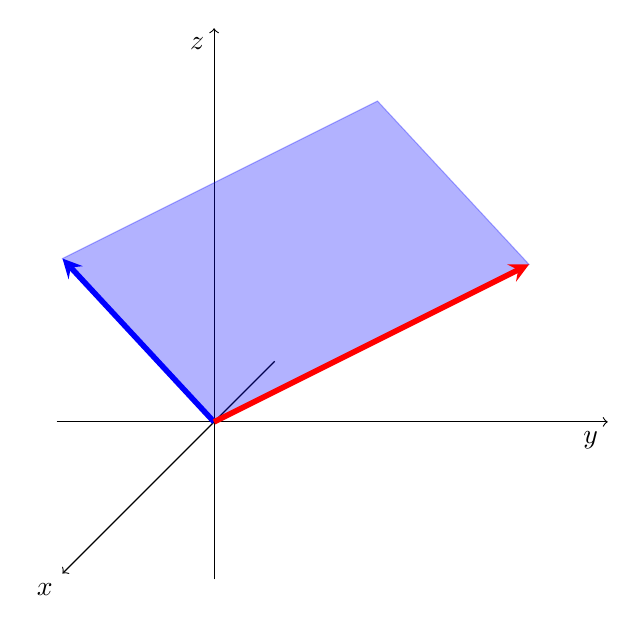
\begin{tikzpicture}
	\draw[->](-2,0,0)--(5,0,0) node[below left]{$y$};
    \draw[->](0,-2,0)--(0,5,0) node[below left]{$z$};
    \draw[->](0,0,-2)--(0,0,5) node[below left]{$x$};
    \filldraw[blue, opacity=0.3] (0,0,0)--(4, 2, 0)--(4,6,5)--(0, 4, 5)--cycle;
    \draw[->, line width=2pt,blue, -stealth](0,0,0)--(0,4,5);
    \draw[->, line width=2pt,red, -stealth](0,0,0)--(4,2,0);
    
\end{tikzpicture}
\end{image}

Because Procedure \ref{pro:lincombgeo} of VEC-M-0040 can be applied to vectors that lie in $p$ just as easily as it can be applied to vectors of $\RR^2$, we conclude that every vector in $p$ can be expressed as a linear combination of $\begin{bmatrix}5\\0\\4\end{bmatrix}$ and  $\begin{bmatrix}0\\4\\2\end{bmatrix}$.  Thus, 

$$\textnormal{span}\left(\begin{bmatrix}5\\0\\4\end{bmatrix}, \begin{bmatrix}0\\4\\2\end{bmatrix}\right)=p$$

\end{explanation}
\end{example}

\section*{Redundant Vectors and Span}

\begin{example}\label{ex:redundantvectors}
We will now revisit Example \ref{ex:spanoftwovectors} and explore what happens when a third vector is introduced into the spanning set $\left\{\begin{bmatrix}5\\0\\4\end{bmatrix}, \begin{bmatrix}0\\4\\2\end{bmatrix}\right\}$  

\begin{enumerate}
\item \label{item:redundantvectors1}
Describe $\textnormal{span}\left(\begin{bmatrix}5\\0\\4\end{bmatrix}, \begin{bmatrix}0\\4\\2\end{bmatrix},\begin{bmatrix}5\\4\\6\end{bmatrix}\right)$.
\item \label{item:redundantvectors2}
Describe $\textnormal{span}\left(\begin{bmatrix}5\\0\\4\end{bmatrix}, \begin{bmatrix}0\\4\\2\end{bmatrix},\begin{bmatrix}4\\5\\0\end{bmatrix}\right)$.
\end{enumerate}
\begin{explanation}
\ref{item:redundantvectors1} From Example \ref{ex:spanoftwovectors}, we know that the first two vectors span a plane in $\RR^3$.  What we have to find out is what, if anything, is accomplished by adding $\begin{bmatrix}5\\4\\6\end{bmatrix}$ to the list.  

By Definition \ref{def:span}, given any vector $\vec{v}$ in $\textnormal{span}\left(\begin{bmatrix}5\\0\\4\end{bmatrix}, \begin{bmatrix}0\\4\\2\end{bmatrix},\begin{bmatrix}5\\4\\6\end{bmatrix}\right)$, we can write $\vec{v}$ as a linear combination of the three vectors in the spanning set
$$\vec{v}=a_1\begin{bmatrix}5\\0\\4\end{bmatrix}+ a_2\begin{bmatrix}0\\4\\2\end{bmatrix}+a_3\begin{bmatrix}5\\4\\6\end{bmatrix}$$

Observe that the third vector is a linear combination of the the first two: $$\begin{bmatrix}5\\4\\6\end{bmatrix}=\begin{bmatrix}5\\0\\4\end{bmatrix}+\begin{bmatrix}0\\4\\2\end{bmatrix}$$

By substitution we obtain
\begin{align*}
\vec{v}&=a_1\begin{bmatrix}5\\0\\4\end{bmatrix}+ a_2\begin{bmatrix}0\\4\\2\end{bmatrix}+a_3\begin{bmatrix}5\\4\\6\end{bmatrix}\\
&=a_1\begin{bmatrix}5\\0\\4\end{bmatrix}+ a_2\begin{bmatrix}0\\4\\2\end{bmatrix}+a_3\left(\begin{bmatrix}5\\0\\4\end{bmatrix}+\begin{bmatrix}0\\4\\2\end{bmatrix}\right)\\
&=(a_1+a_3)\begin{bmatrix}5\\0\\4\end{bmatrix}+ (a_2+a_3)\begin{bmatrix}0\\4\\2\end{bmatrix}
\end{align*} 
Thus, $\vec{v}$ is in $\textnormal{span}\left(\begin{bmatrix}5\\0\\4\end{bmatrix}, \begin{bmatrix}0\\4\\2\end{bmatrix}\right)$. 

We conclude that all vectors in $\textnormal{span}\left(\begin{bmatrix}5\\0\\4\end{bmatrix}, \begin{bmatrix}0\\4\\2\end{bmatrix},\begin{bmatrix}5\\4\\6\end{bmatrix}\right)$ are also in $\textnormal{span}\left(\begin{bmatrix}5\\0\\4\end{bmatrix}, \begin{bmatrix}0\\4\\2\end{bmatrix}\right)$.  

Moreover, every vector in $\textnormal{span}\left(\begin{bmatrix}5\\0\\4\end{bmatrix}, \begin{bmatrix}0\\4\\2\end{bmatrix}\right)$ is clearly in $\textnormal{span}\left(\begin{bmatrix}5\\0\\4\end{bmatrix}, \begin{bmatrix}0\\4\\2\end{bmatrix},\begin{bmatrix}5\\4\\6\end{bmatrix}\right)$.
Thus,
$$\textnormal{span}\left(\begin{bmatrix}5\\0\\4\end{bmatrix}, \begin{bmatrix}0\\4\\2\end{bmatrix},\begin{bmatrix}5\\4\\6\end{bmatrix}\right)=\textnormal{span}\left(\begin{bmatrix}5\\0\\4\end{bmatrix}, \begin{bmatrix}0\\4\\2\end{bmatrix}\right)$$

Geometrically, $\begin{bmatrix}5\\4\\6\end{bmatrix}$ is the diagonal of a parallelogram determined by $\begin{bmatrix}0\\4\\2\end{bmatrix}$ and  $\begin{bmatrix}5\\0\\4\end{bmatrix}$, and lies in the plane spanned by these vectors. This relationship is illustrated by the diagram below.


\begin{image}
\tdplotsetmaincoords{70}{130}
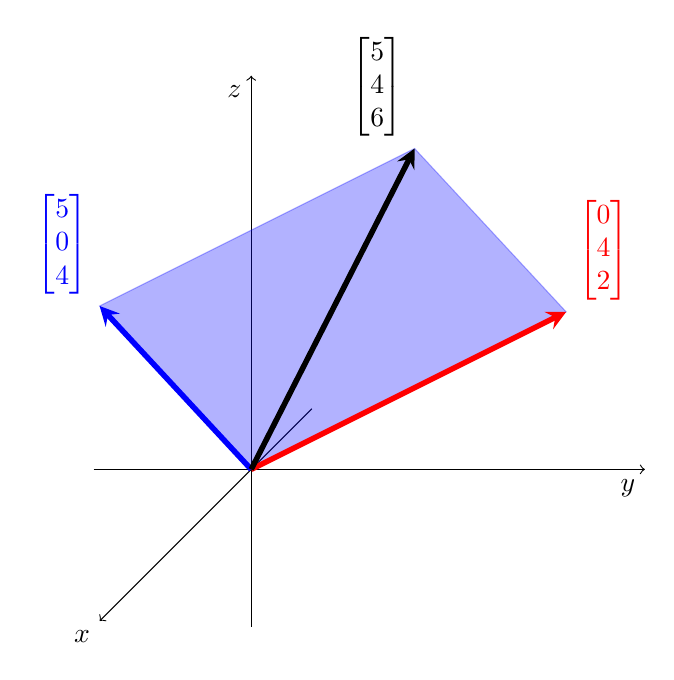
\begin{tikzpicture}
	\draw[->](-2,0,0)--(5,0,0) node[below left]{$y$};
    \draw[->](0,-2,0)--(0,5,0) node[below left]{$z$};
    \draw[->](0,0,-2)--(0,0,5) node[below left]{$x$};
    \filldraw[blue, opacity=0.3] (0,0,0)--(4, 2, 0)--(4,6,5)--(0, 4, 5)--cycle;
    \draw[->, line width=2pt,blue, -stealth](0,0,0)--(0,4,5)node[above left]{$\begin{bmatrix}5\\0\\4\end{bmatrix}$};
    \draw[->, line width=2pt,red, -stealth](0,0,0)--(4,2,0)node[above right]{$\begin{bmatrix}0\\4\\2\end{bmatrix}$};
    \draw[->, line width=2pt, -stealth](0,0,0)--(4,6,5)node[above left]{$\begin{bmatrix}5\\4\\6\end{bmatrix}$};
    
\end{tikzpicture}
\end{image}

Every vector in $\textnormal{span}\left(\begin{bmatrix}5\\0\\4\end{bmatrix}, \begin{bmatrix}0\\4\\2\end{bmatrix},\begin{bmatrix}5\\4\\6\end{bmatrix}\right)$ lies in this plane.

\ref{item:redundantvectors2}
We will consider this problem from the geometric standpoint first.  The three vectors are shown in the diagram below together with the plane that is the span of $\begin{bmatrix}5\\0\\4\end{bmatrix}$ and $\begin{bmatrix}0\\4\\2\end{bmatrix}$.
\begin{image}
\tdplotsetmaincoords{70}{130}
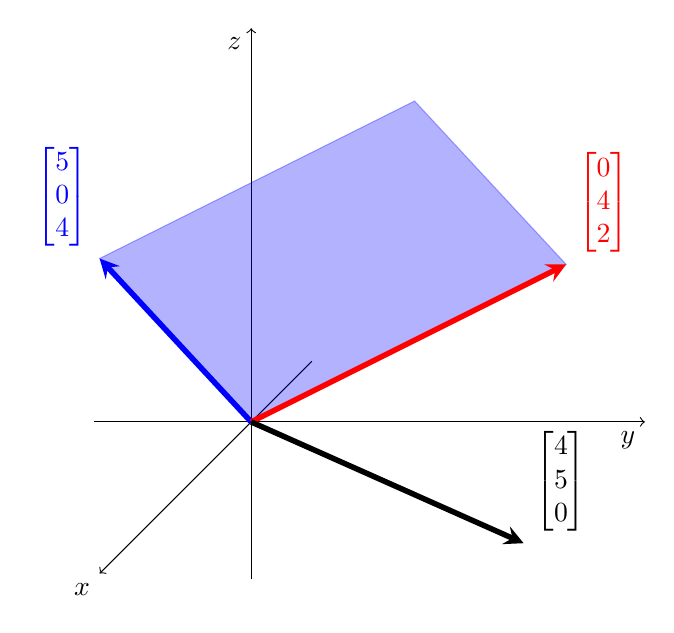
\begin{tikzpicture}
	\draw[->](-2,0,0)--(5,0,0) node[below left]{$y$};
    \draw[->](0,-2,0)--(0,5,0) node[below left]{$z$};
    \draw[->](0,0,-2)--(0,0,5) node[below left]{$x$};
    \filldraw[blue, opacity=0.3] (0,0,0)--(4, 2, 0)--(4,6,5)--(0, 4, 5)--cycle;
    \draw[->, line width=2pt,blue, -stealth](0,0,0)--(0,4,5)node[above left]{$\begin{bmatrix}5\\0\\4\end{bmatrix}$};
    \draw[->, line width=2pt,red, -stealth](0,0,0)--(4,2,0)node[above right]{$\begin{bmatrix}0\\4\\2\end{bmatrix}$};
    \draw[->, line width=2pt, -stealth](0,0,0)--(5,0,4)node[above right]{$\begin{bmatrix}4\\5\\0\end{bmatrix}$};
    
\end{tikzpicture}
\end{image}
Considering that the three vectors lie in three different coordinate planes (why?), it is easy to see that they do not lie in the same plane.  This shows that 
$$\textnormal{span}\left(\begin{bmatrix}5\\0\\4\end{bmatrix}, \begin{bmatrix}0\\4\\2\end{bmatrix},\begin{bmatrix}4\\5\\0\end{bmatrix}\right)\neq\textnormal{span}\left(\begin{bmatrix}5\\0\\4\end{bmatrix}, \begin{bmatrix}0\\4\\2\end{bmatrix}\right)$$

We will now show that 
$$\textnormal{span}\left(\begin{bmatrix}5\\0\\4\end{bmatrix}, \begin{bmatrix}0\\4\\2\end{bmatrix},\begin{bmatrix}4\\5\\0\end{bmatrix}\right)=\RR^3$$

To do this, consider an arbitrary vector $\vec{u}=\begin{bmatrix}s\\t\\r\end{bmatrix}$ in $\RR^3$.  We need to show that $\vec{u}$ is a linear combination of 

$$\begin{bmatrix}5\\0\\4\end{bmatrix}, \begin{bmatrix}0\\4\\2\end{bmatrix},\begin{bmatrix}4\\5\\0\end{bmatrix}$$

We can do this by solving a vector equation
$$a_1\begin{bmatrix}5\\0\\4\end{bmatrix}+ a_2\begin{bmatrix}0\\4\\2\end{bmatrix}+a_3\begin{bmatrix}4\\5\\0\end{bmatrix}=\begin{bmatrix}s\\t\\r\end{bmatrix}$$
This vector equation corresponds to a linear system that can be written in augmented matrix form and reduced as follows:
\begin{align}\label{eq:gjreductionspan}\left[\begin{array}{ccc|c}  
 5&0&4&s\\0&4&5&t\\4&2&0&r
 \end{array}\right]\rightsquigarrow\left[\begin{array}{ccc|c}  
 1&0&0&\star\\0&1&0&\star\\0&0&1&\star
 \end{array}\right]\end{align}
 
 While we chose not to keep track of the entries on the right-hand side, it is clear that these entries will be real numbers. (You will be asked to fill in the details in Practice Problem {\color{red} reference}.)  We conclude that every vector of $\RR^3$ can be written as a linear combination of the three vectors.  Therefore 
 $$\textnormal{span}\left(\begin{bmatrix}5\\0\\4\end{bmatrix}, \begin{bmatrix}0\\4\\2\end{bmatrix},\begin{bmatrix}4\\5\\0\end{bmatrix}\right)=\RR^3$$
\end{explanation}
\end{example}

In part \ref{item:redundantvectors1} of Example \ref{ex:redundantvectors} we saw that adding $\begin{bmatrix}5\\4\\6\end{bmatrix}$ to the spanning set does not change the span.  We observed that this phenomenon is due to the fact that $\begin{bmatrix}5\\4\\6\end{bmatrix}$ is a linear combination of the other two vectors in the spanning set.

Because
$\textnormal{span}\left(\begin{bmatrix}5\\0\\4\end{bmatrix}, \begin{bmatrix}0\\4\\2\end{bmatrix},\begin{bmatrix}5\\4\\6\end{bmatrix}\right)=\textnormal{span}\left(\begin{bmatrix}5\\0\\4\end{bmatrix}, \begin{bmatrix}0\\4\\2\end{bmatrix}\right)$,
we say that $\begin{bmatrix}5\\4\\6\end{bmatrix}$ is \dfn{redundant}.  

%In fact, each vector in the spanning set
%$$\left\{\begin{bmatrix}5\\0\\4\end{bmatrix}, \begin{bmatrix}0\\4\\2\end{bmatrix},\begin{bmatrix}5\\4\\6\end{bmatrix}\right\}$$
%is redundant because removing any one of them does not change the span.

In part \ref{item:redundantvectors2}, adding the vector $\begin{bmatrix}4\\5\\0\end{bmatrix}$ to the spanning set did change the span. The set 
$$\left\{\begin{bmatrix}5\\0\\4\end{bmatrix}, \begin{bmatrix}0\\4\\2\end{bmatrix},\begin{bmatrix}4\\5\\0\end{bmatrix}\right\}$$ does not contain redundant vectors.

\begin{definition}\label{def:redundant}
Given a set of vectors $\{\vec{v}_1,\vec{v}_2,\ldots ,\vec{v}_p\}$ an element $\vec{v}_i$ of the set is called \dfn{redundant} if $\vec{v}_i$ can be expressed as a linear combination of the other elements of the set.  
\end{definition}

\begin{example} Vector $\begin{bmatrix}0\\4\end{bmatrix}$ of $\left\{\begin{bmatrix}1\\-3\end{bmatrix},\begin{bmatrix}0\\4\end{bmatrix}, \begin{bmatrix}0\\-2\end{bmatrix}\right\}$ is redundant because it can be expressed as a linear combination of the remaining vectors:  
$$0\begin{bmatrix}1\\-3\end{bmatrix}+(-2)\begin{bmatrix}0\\-2\end{bmatrix}= \begin{bmatrix}0\\4\end{bmatrix}$$

We may also say that the vector $\begin{bmatrix}0\\-2\end{bmatrix}$ is redundant because
$$0\begin{bmatrix}1\\-3\end{bmatrix}+\left(-\frac{1}{2}\right)\begin{bmatrix}0\\4\end{bmatrix}= \begin{bmatrix}0\\-2\end{bmatrix}$$
\end{example}



\section*{Practice Problems}

\begin{problem}
Choose the best description for each set below.
  \begin{problem}
  $$\textnormal{span}\left(\begin{bmatrix}1\\1\\-2\end{bmatrix}, \begin{bmatrix}2\\2\\-4\end{bmatrix}\right)$$
  
  \begin{multipleChoice}
 \choice{Plane in $\RR^3$}
 \choice{Line in $\RR^2$}
     \choice[correct]{Line in $\RR^3$}
 \choice{$\RR^3$}
  \choice{$\RR^2$ }
 \end{multipleChoice}
  \end{problem}
  
  \begin{problem}
  $$\textnormal{span}\left(\begin{bmatrix}1\\-2\end{bmatrix}, \begin{bmatrix}1\\0\end{bmatrix}\right)$$
  
   \begin{multipleChoice}
 \choice{Plane in $\RR^3$}
 \choice{Line in $\RR^2$}
     \choice{Line in $\RR^3$}
 \choice{$\RR^3$}
  \choice[correct]{$\RR^2$ }
  
\end{multipleChoice}
  \end{problem}
  \begin{problem}
  $$\textnormal{span}\left(\begin{bmatrix}-3\\1\end{bmatrix}, \begin{bmatrix}6\\-2\end{bmatrix}, \begin{bmatrix}3\\-1\end{bmatrix}\right)$$
  
  \begin{multipleChoice}
 \choice{Plane in $\RR^3$}
 \choice[correct]{Line in $\RR^2$}
     \choice{Line in $\RR^3$}
 \choice{$\RR^3$}
  \choice{$\RR^2$ }
  
\end{multipleChoice}
  
  \end{problem}
\end{problem}
\begin{problem}
Which of the following pairs of sets are equal?  

\begin{selectAll}
  \choice[correct]{$V=\textnormal{span}\left(\begin{bmatrix}5\\0\\0\end{bmatrix},\begin{bmatrix}10\\0\\0\end{bmatrix},\begin{bmatrix}0\\0\\-4\end{bmatrix}\right)\quad\text{and}\quad W=\textnormal{span}\left(\begin{bmatrix}-2\\0\\0\end{bmatrix},\begin{bmatrix}0\\0\\1\end{bmatrix}\right)$}
 \choice[correct]{$V=\textnormal{span}\left(\begin{bmatrix}5\\3\end{bmatrix},\begin{bmatrix}10\\-1\end{bmatrix},\begin{bmatrix}0\\2\end{bmatrix}\right)\quad\text{and}\quad W=\textnormal{span}\left(\begin{bmatrix}-2\\0\end{bmatrix},\begin{bmatrix}0\\1\end{bmatrix}\right)$}
 \choice{$V=\textnormal{span}\left(\begin{bmatrix}1\\-2\\4\end{bmatrix}\right)\quad\text{and}\quad W=\textnormal{span}\left(\begin{bmatrix}-1\\2\\-4\end{bmatrix},\begin{bmatrix}0\\0\\1\end{bmatrix}\right)$}
 \choice[correct]{$V=\textnormal{span}\left(\begin{bmatrix}5\\0\end{bmatrix}\right)\quad\text{and}\quad W=\textnormal{span}\left(\begin{bmatrix}-2\\0\end{bmatrix},\begin{bmatrix}1\\0\end{bmatrix},\begin{bmatrix}-4\\0\end{bmatrix},\begin{bmatrix}0\\0\end{bmatrix}\right)$}
\end{selectAll}
\end{problem}

\begin{problem}
Let $\vec{v}=\begin{bmatrix}3\\4\\5\end{bmatrix}$.  Give an example of at least one vector $\vec{w}$ such that $\vec{v}$, $\vec{w}$ do NOT span a plane in $\RR^3$.  Describe $\textnormal{span}(\vec{v}, \vec{w})$.
\end{problem}

\begin{problem}Does the given set contain redundant vectors?  If so, express one of the vectors in the set as a linear combination of the others.
\begin{problem}
  $$\left\{\begin{bmatrix}-2\\4\end{bmatrix},\begin{bmatrix}1\\2\end{bmatrix}\right\}$$
  \end{problem}
  
  \begin{problem}
  $$\left\{\begin{bmatrix}0\\-3\end{bmatrix},\begin{bmatrix}2\\-1\end{bmatrix}\right\}$$
  \end{problem}

  \begin{problem}
  $$\left\{\begin{bmatrix}-2\\4\\1\end{bmatrix},\begin{bmatrix}1\\5\\2\end{bmatrix}, \begin{bmatrix}5\\-3\\0\end{bmatrix}\right\}$$
  \end{problem}
  
\end{problem}

\begin{problem} Supply the steps in the row reduction process in (\ref{eq:gjreductionspan}) and express $\begin{bmatrix}s\\t\\r\end{bmatrix}$ as a linear combination of $$\begin{bmatrix}5\\0\\4\end{bmatrix},\begin{bmatrix}0\\4\\2\end{bmatrix},\begin{bmatrix}4\\5\\0\end{bmatrix}$$
\end{problem}


\begin{problem}Prove or disprove.  The zero vector of $\RR^n$ is contained in the span of any collection of vectors of $\RR^n$.
\end{problem}

\begin{problem}
Let $\vec{v}_1,\vec{v}_2,\ldots ,\vec{v}_p$ be vectors of $\RR^n$.  Prove that for any collection of scalars $a_1, a_2,\ldots ,a_p$ 
$$\textnormal{span}(\vec{v}_1,\vec{v}_2,\ldots ,\vec{v}_p)=\textnormal{span}(\vec{v}_1,\vec{v}_2,\ldots ,\vec{v}_p,a_1\vec{v}_1+a_2\vec{v}_2+\ldots +a_p\vec{v}_p)$$
In other words, show that adding a linear combination of vectors in a spanning set to the spanning set does not change the span.
\end{problem}

%\begin{problem} In Example \ref{ex:sapnoftwovectors} we said that $\begin{bmatrix}5\\0\\4\end{bmatrix}, \begin{bmatrix}0\\4\\2\end{bmatrix}$ ``determine a plane".  What does this statement mean?  Can you think of two vectors that do not determine a plane?
%\end{problem}


\end{document} 